\documentclass{article}
\usepackage{graphicx} % Required for inserting images





\documentclass[a4paper,12pt]{article}
\usepackage[utf8]{inputenc}
\usepackage{graphicx}
%  Русский язык
\usepackage{multirow}
\usepackage{wrapfig}
\usepackage[T2A]{fontenc}			% кодировка
\usepackage[utf8]{inputenc}			% кодировка исходного текста
\usepackage[english,russian]{babel}	% локализация и переносы

\usepackage{indentfirst} %Красная строка
\usepackage[a4paper,top=1.3cm,bottom=2cm,left=1.5cm,right=1.5cm,marginparwidth=0.5cm]{geometry}
\usepackage[usenames]{color}
\usepackage{colortbl}
\usepackage{csvsimple}
\usepackage{siunitx}
\usepackage{graphicx}
\graphicspath{ {images/} }
\usepackage{tikz}
\usepackage{pgfplots}

\usepackage{amsmath}
\usepackage{floatflt}
\usepackage[left=20mm, top=20mm, right=20mm, bottom=20mm, footskip=10mm]{geometry}

\usepackage{multicol}
\setlength{\columnsep}{2cm}

\usepackage{multicol}
\setlength{\columnsep}{2cm}
\usepackage{hyperref}


% Заметки
\usepackage{todonotes}

% Математика
\usepackage{amsmath,amsfonts,amssymb,amsthm,mathtools} 
\usepackage{hyperref}

\renewcommand{\AA}{\ensuremath{\mathring{A}}}

\begin{document}
\def\figurename{Рисунок}
\begin{titlepage}
\begin{center}
    {\large МОСКОВСКИЙ ФИЗИКО-ТЕХНИЧЕСКИЙ ИНСТИТУТ (НАЦИОНАЛЬНЫЙ ИССЛЕДОВАТЕЛЬСКИЙ УНИВЕРСИТЕТ)}
\end{center}
\begin{center}
    {\largeФизтех-школа биологической и медицинской физики}
\end{center}

\vspace{1cm}
{\huge
\begin{center}
    {\bf Лабораторная работа по общей физике}\\
    \vspace{0.5cm}
    4.3.2 Дифракция света на ультразвуковой волне в жидкости
\end{center}
}

\vspace{4cm}
\begin{flushright}
{\LARGE Выполнила студентка группы Б06-103:\\ Фитэль Алена \\}

\end{flushright}
\vspace{9cm}
\begin{center}
    Долгопрудный, 2023 г.
\end{center}
\end{titlepage}
\newpage
\section{Введение}

\textbf{Цель работы:}  изучение дифракции света на синусоидальной акустической решетке и наблюдение фазовой решетки методом темного поля.

\textbf{В работе используются:} оптическая скамья, осветитель, два длиннофокусных объектива, кювета с жидкостью, кварцевый излучатель с микрометрическим винтом, генератор звуковой частоты, линза, вертикальная нить на рейтере, микроскоп.

\section{Теоретические сведения}

При прохождении ультразвуковой волны через жидкость в ней возникают периодические неоднородности коэффициента преломления, создается фазовая решетка, которую мы считаем неподвижной ввиду малости скорости звука относительно скорости света. Показатель
	преломления n изменяется по закону:
	
	\begin{equation}\label{}
	n = n_0 (1 + m \cos \Omega x)
	\end{equation}
	
	Здесь $ \Omega = 2 \pi / \Lambda $ --- волновое число для ультразвуковой волны, $ m $ --- глубина модуляции $ n $ $ (m \ll 1 $).
	
	Положим фазу $ \phi $ колебаний световой волны на передней стенке кюветы равной нулю, тогда на задней поверхности она равна:
	
	\begin{equation}\label{}
	\phi  = k n L = \phi_0 (1 + m \cos \Omega x)
	\end{equation}
	
	Здесь $ L $ --- толщина жидкости в кювете, $ k = 2 \pi / \lambda $ --- волновое число для света.
	
	После прохождения через кювету световое поле есть совокупность плоских волн, распространяющихся под углами $ \theta $, соответствующими максимумам в дифракции Фраунгофера:
	
\begin{equation}\label{}	
	\Lambda \sin \theta_m = m \lambda
\end{equation}

	Этот эффект проиллюстрирован на рисунке 1.



 \begin{figure}[h!]
	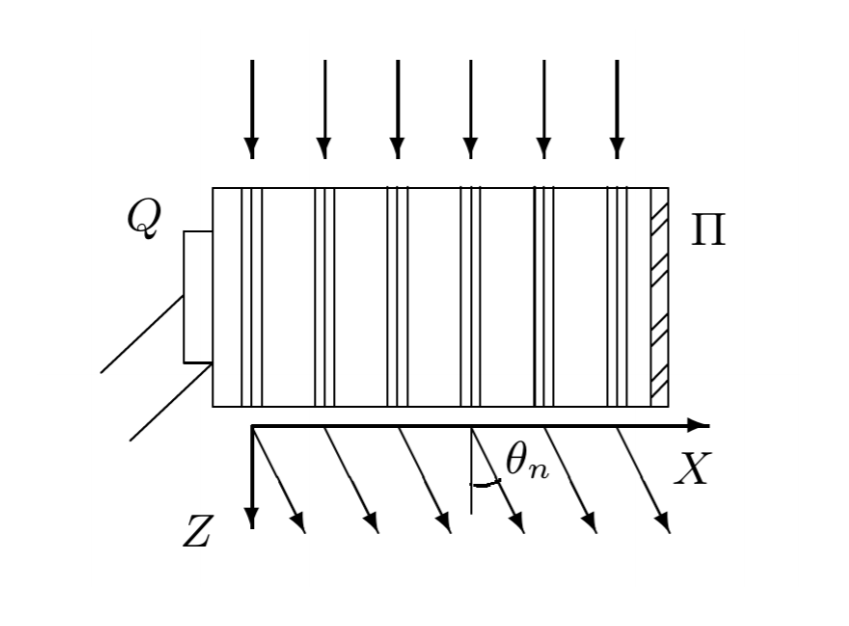
\includegraphics[scale=0.23]{wave.png}
	\centering
	\caption{Дифракция световых волн на акустической решетке}
\end{figure}

    Зная положение дифракционных максимумов, по формуле (1) легко определить длину ультразвуковой волны, учитывая малость $ \theta $: $ \sin \theta \approx \theta \approx l_m /F  $, где $ l_m $ --- расстояние от нулевого до последнего видимого максимума, $ F $ --- фокусное расстояние линзы. Тогда получим:
    	
    	\begin{equation}\label{}
    	 \Lambda = m \lambda F/ l_m 
    	\end{equation}
    	Скорость ультразвуковых волн в жидкости, где $ \nu $ --- частота колебаний излучателя:
    	
    \begin{equation}\label{}
    	v = \Lambda \nu 
    \end{equation}
    
    \textbf{Схема установки. }Схема установки приведена на рисунке 2. Источник света Л через светофильтр Ф и конденсор К освещает вертикальную щель $ S $, находящуюся в фокусе объектива $ O_1 $. После объектива параллельный световой пучок проходит через кювету С перпендикулярно акустической решетке, и дифракционная картина собирается в фокальной плоскости объектива $ O_2 $ , наблюдается при помощи микроскопа М.

    Предварительную настройку установки произведем в соответствии с инструкцией с зеленым фильтром, далее в работе используется красный.
    
\begin{figure}[h!]
	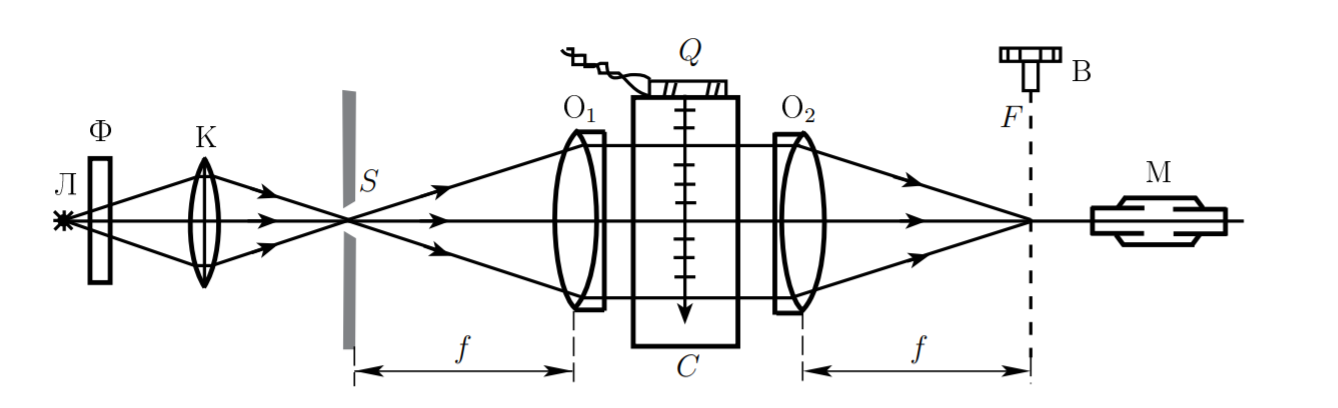
\includegraphics[scale=0.3]{stand.png}
	\centering
	\caption{Схема для наблюдения дифракции на акустической решетке}
\end{figure}

 Параметры установки: фокусное расстояние объектива $F = 30 $ см, одно деление винта микроскопа составляет 20~мкм, полоса пропускания фильтра \mbox{$\lambda = 6400\pm 200$ Å}.
 \\ Во второй части работы будет использован метод темного поля для определения скорости ультразвука. Для этого изменим изначальную схему
согласно Рисунку 3.
 \begin{figure}[h!]
	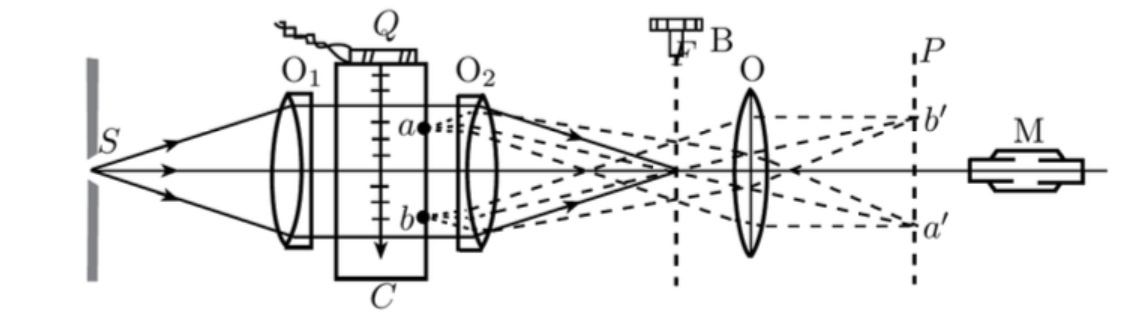
\includegraphics[scale=0.3]{tteo.jpg}
	\centering
	\caption{Схема для наблюдения акустической решетки методом темного поля }
\end{figure}
	
\section{Обработка результатов}
\subsection{Определение скорости ультразвука по дифракционной картине}
\begin{enumerate}

  \item  Измерим положения $ x_m $ дифракционных максимумов с помощью микроскопического винта для четырех частот. Результаты измерений приведены в Таблице 1. На основе таблицы для каждой из частот проведем линейную аппроксимацию зависимости $ x_m (m) $ (Рисунок 3). 

\begin{table}[h!]
\centering
\begin{tabular}{|l|c|l|l|l|l|l|l|l|l|l|}
\hline
$\nu, \text{МГц}$ & \textbf{$m$} & \multicolumn{1}{c|}{\textbf{-4}} & \multicolumn{1}{c|}{\textbf{-3}} & \multicolumn{1}{c|}{-2}   & \multicolumn{1}{c|}{-1}   & \multicolumn{1}{c|}{0}    & \multicolumn{1}{c|}{1}    & \multicolumn{1}{c|}{2}    & \multicolumn{1}{c|}{3}    & \multicolumn{1}{c|}{4}    \\ \hline
1,17              & $x_m, \
text{мкм}$ & \multicolumn{1}{c|}{450}         & \multicolumn{1}{c|}{730}         & \multicolumn{1}{c|}{1080} & \multicolumn{1}{c|}{1370} & \multicolumn{1}{c|}{1730} & \multicolumn{1}{c|}{2060} & \multicolumn{1}{c|}{2360} & \multicolumn{1}{c|}{2700} & \multicolumn{1}{c|}{2950} \\ \cline{1-1} \cline{3-11} 
1,82              &              & -                                & 50                               & 460                       & 1150                      & 1590                      & 2110                      & 2710                      & 3280                      & -                         \\ \cline{1-1} \cline{3-11} 
1,55              &              & -                                & 460                              & 790                       & 1230                      & 1610                      & 2030                      & 2540                      & 3000                      & -                         \\ \cline{1-1} \cline{3-11} 
3,96              &              & -                                & -                                & 440                       & 1500                      & 2790                      & 3730                      & 5070                      & -                         & -                         \\ \hline
\end{tabular}
\caption{Измерение координаты m-го максимума дифракционной картины для разных частот}
\label{tab:my-table}
\end{table}


  \begin{figure}[h!]
	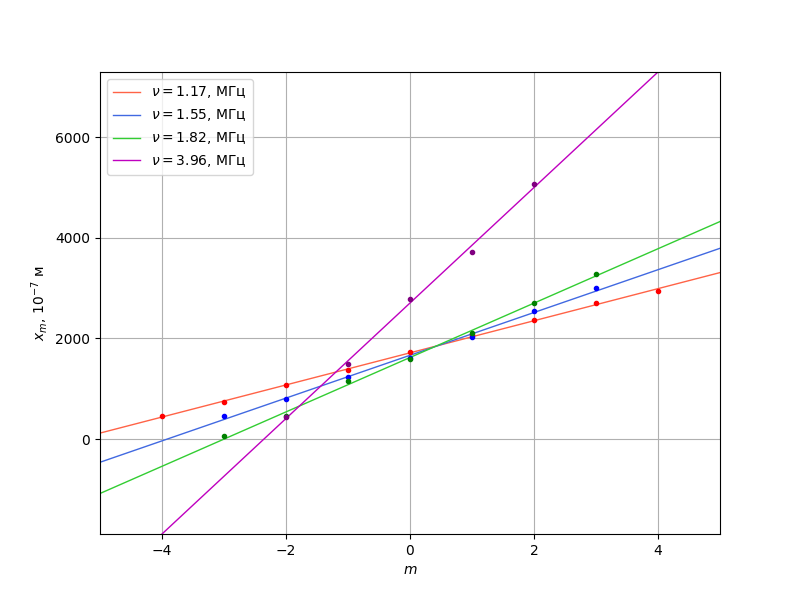
\includegraphics[scale=0.8]{Figure_1!!!.png}
	\centering
	\caption{Графики зависимостей $x_m(m)$ для разных частот }
\end{figure}


 \item  По полученным коэффициентам наклона графика определим для каждой частоты $l_m/m$, и по формуле (4) рассчитаем длины волн $\Lambda$ для всех частот. Резульатыт приведены в Таблице 2.
 \begin{table}[h!]
\centering
\begin{tabular}{|c|c|c|c|c|}
\hline
$\nu$, МГц     & \textbf{1.17} & \textbf{1.55} & \textbf{1.82} & 3.96   \\ \hline
$l_m/m$, мкм   & 133.04        & 177.38        & 225.41        & 478.75 \\ \hline
$\Lambda$, мкм & 1343          & 1082          & 852           & 401    \\ \hline
\end{tabular}
\caption{Длины волн для разных частот}
\label{tab:my-table}
\end{table}
\item	Построим график $\Lambda(1/\nu)$. По коэффициенту наклона определим скорость ультразвука в воде из формулы (5):
	$$v=1591\pm52\text{ м/с}.$$
Для сравнения табличное значение составляет $v=1490$ м/с
  \begin{figure}[h!]
	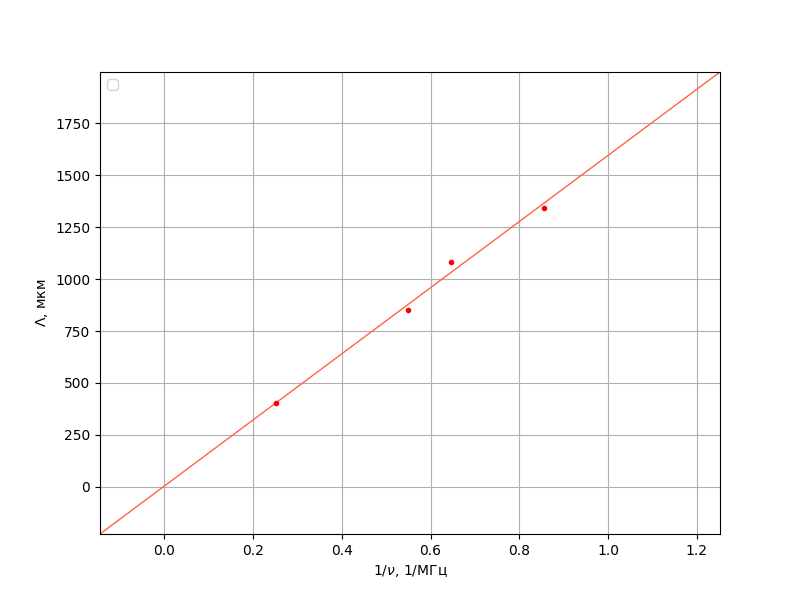
\includegraphics[scale=0.7]{Figure_2!.png}
	\centering
	\caption{Графики зависимости длин УЗ-волн от частоты }
\end{figure}	


\end{enumerate}
\newpage

\subsection{Определение скорости ультразвука методом темного экрана}
\begin{enumerate}

 \item  Приставим к задней стенке (для светового луча) кюветы стеклянную пластинку с миллиметровыми делениями; сфокусируем микроскоп на изображение пластинки. Определим цену деления окулярной шкалы микроскопа, совместив ее с миллиметровыми делениями: цена деления окулярной шкалы: $ C = $ 0,60 \pm 0,02 мм.

  \item  Без применения метода темного поля звуковая решетка не наблюдается. Закроем нулевой максимум горизонтальной нитью. Таким образом, осевая составляющая фазово-модулированной волны поглощается, а боковые остаются без изменения. Получившееся поле: 

\begin{equation}\label{}
f(x) = \dfrac{im}{2} e^{i\Omega x} +  \dfrac{im}{2} e^{-i\Omega x} = im \cos \Omega x; I(x) = m^2 \cos ^2 \Omega x = m^2 \dfrac{1 + \cos ^2 2 \Omega x}{2}
\end{equation}

Отсюда получаем, что расстояние между темными полосами есть $ \Lambda/2 $.

Формулы для расчета длины волны ультразвука $ \Lambda $ и скорости распространения $ v $ в воде:
\begin{equation}\label{}
\Lambda/2  = NC/(n - 1),  \qquad v = \nu\Lambda
\end{equation}

 \item  Проведем измерение длины ультразвуковой волны. Полученные данные и проведенные расчеты преставленны в Таблице 3.

\begin{table}[h!]
\centering
\begin{tabular}{|r|r|r|r|r|l|l|}
\hline
\multicolumn{1}{|l|}{$\nu$, $\text{ МГц}$} & \multicolumn{1}{l|}{\begin{tabular}[c]{@{}l@{}}Количество делений\\ шкалы окуляра,  N\end{tabular}} & \multicolumn{1}{l|}{\begin{tabular}[c]{@{}l@{}}Количество темных полос\\  акустической решетки, n\end{tabular}} & \multicolumn{1}{l|}{\begin{tabular}[c]{@{}l@{}}$\Lambda$,\\  $\text{ мм}$\end{tabular}} & \multicolumn{1}{l|}{v, $\text{ м/c}$} & \begin{tabular}[c]{@{}l@{}}$\delta \Lambda, \\ \text{ мм}$\end{tabular} & \begin{tabular}[c]{@{}l@{}}$\delta v, \\ \text{ м/c}$\end{tabular} \\ \hline
1.2                                        & 100                                                                                                 & 11                                                                                                              & 1.2                                                                                     & 1440                                  & 0.03                                                                    & 36                                                                 \\ \hline
1.56                                       & 100                                                                                                 & 13                                                                                                              & 1.0                                                                                     & 1560                                  & 0.03                                                                    & 47                                                                 \\ \hline
\end{tabular}
\caption{Вычисление длины ультразвуковой волны и ее скорости распространения в воде методом темного поля.}
\label{tab:my-table}
\end{table}


Усреднив результат получим: $v = 1500 \pm 42 \text{ м/с}$. 


\

\newline


\begin{minipage}{0.47\textwidth}
\begin{center}
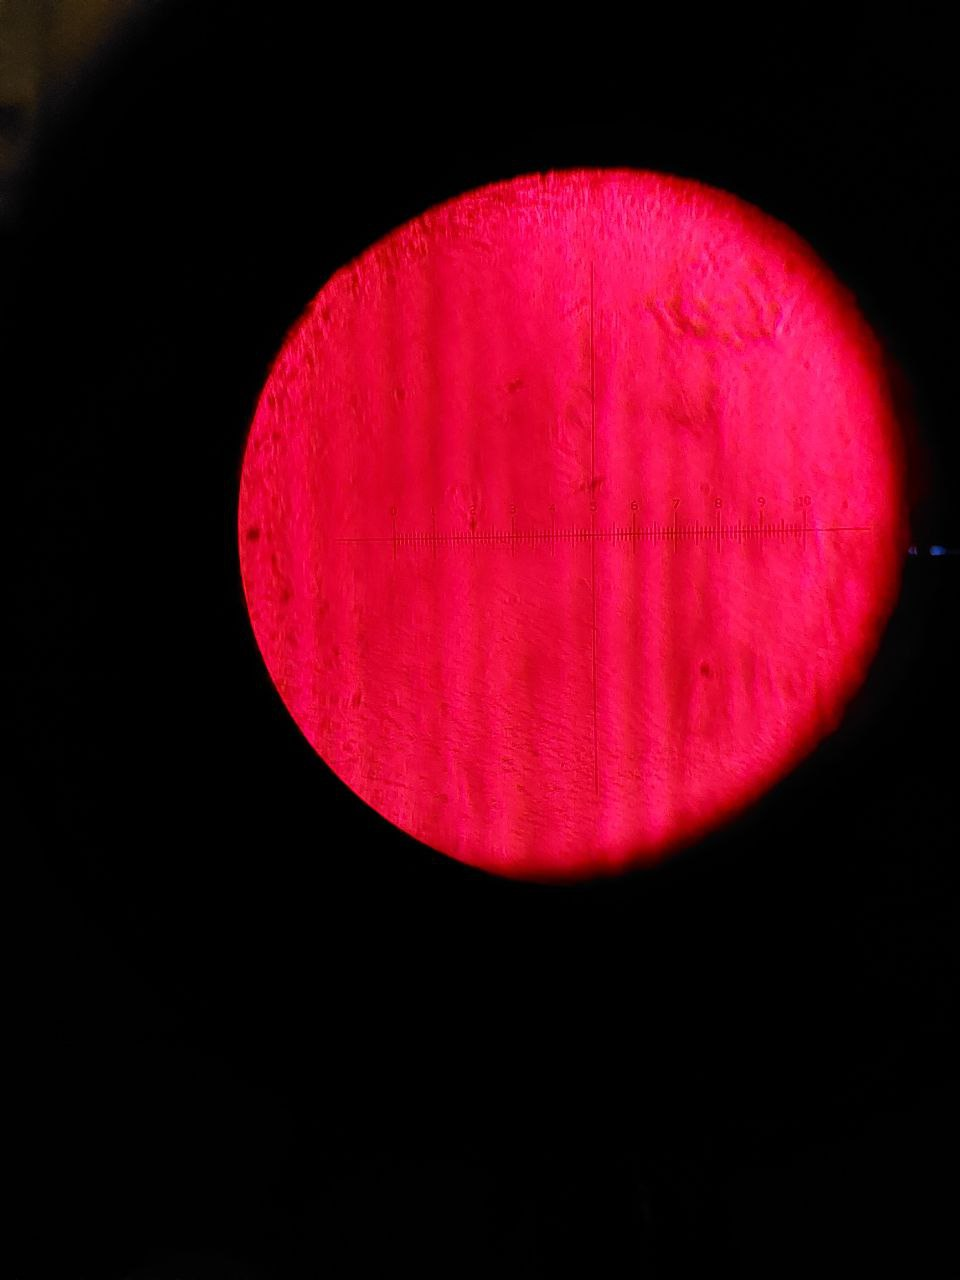
\includegraphics[width=0.7\textwidth]{red 1.jpg}
	
	Наблюдаемая картина при частоте\\ 1.20 МГц.
\end{center}
\end{minipage}
\begin{minipage}{0.47\textwidth}
\begin{center}
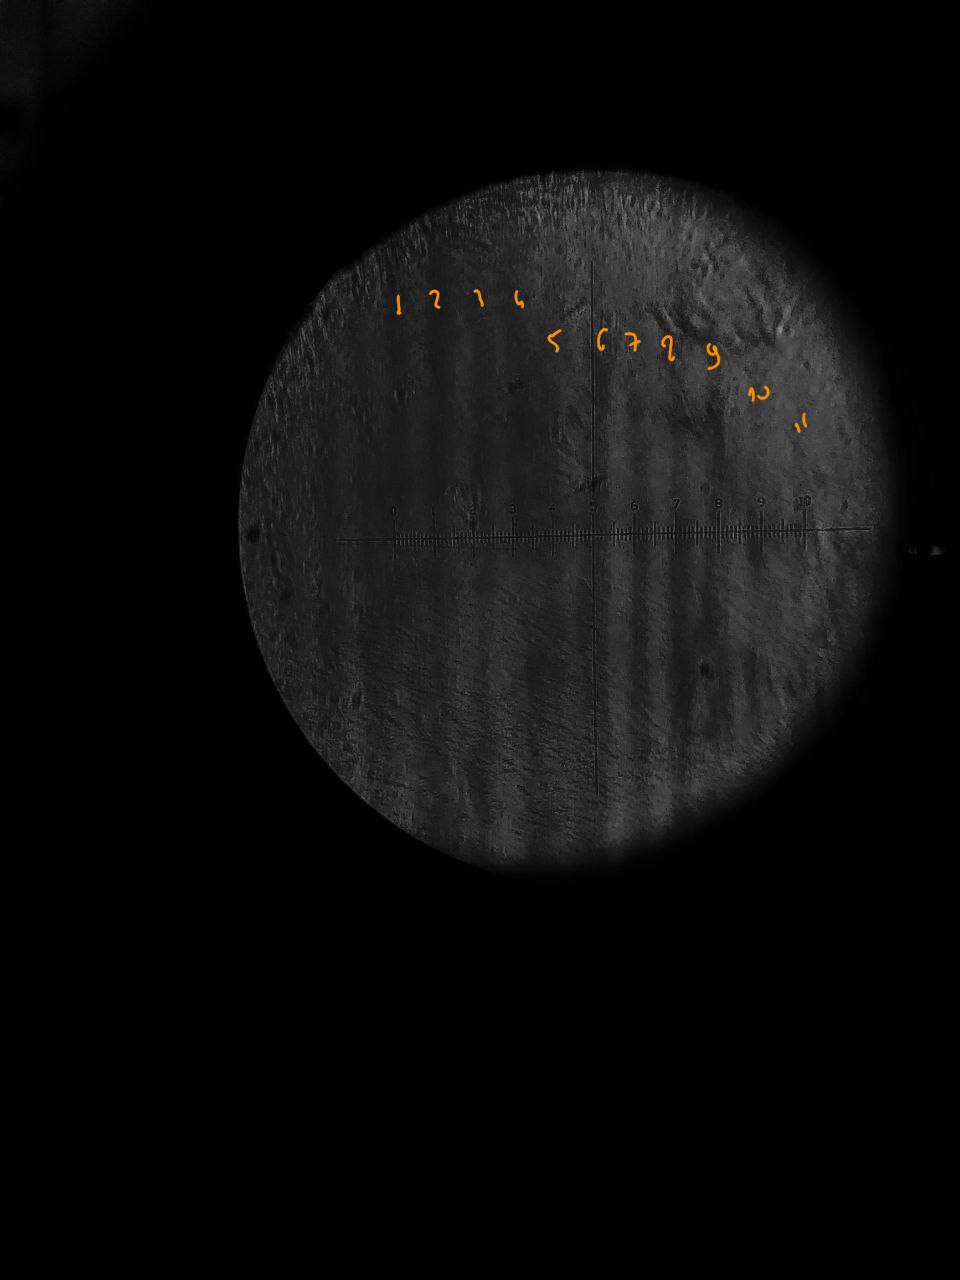
\includegraphics[width=0.7\textwidth]{grey 1.jpg}
	
	Наблюдаемая картина при частоте\\ 1.20 МГц в контрасте.
\end{center}
\end{minipage}

\newline


\begin{minipage}{0.47\textwidth}
\begin{center}
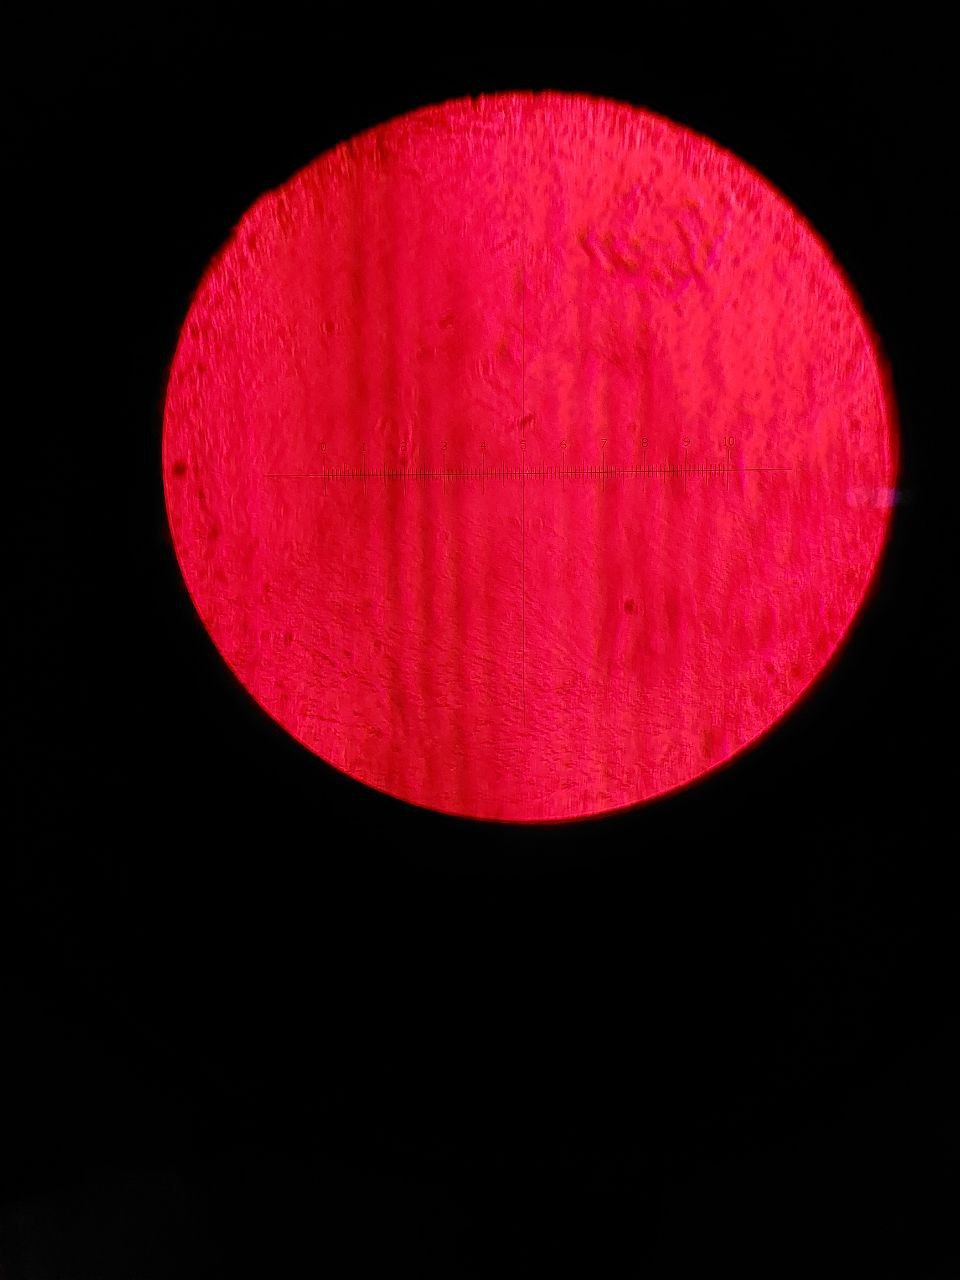
\includegraphics[width=0.7\textwidth]{red 2.jpg}
	
	Наблюдаемая картина при частоте\\ 1.20 МГц.
\end{center}
\end{minipage}
\begin{minipage}{0.47\textwidth}
\begin{center}
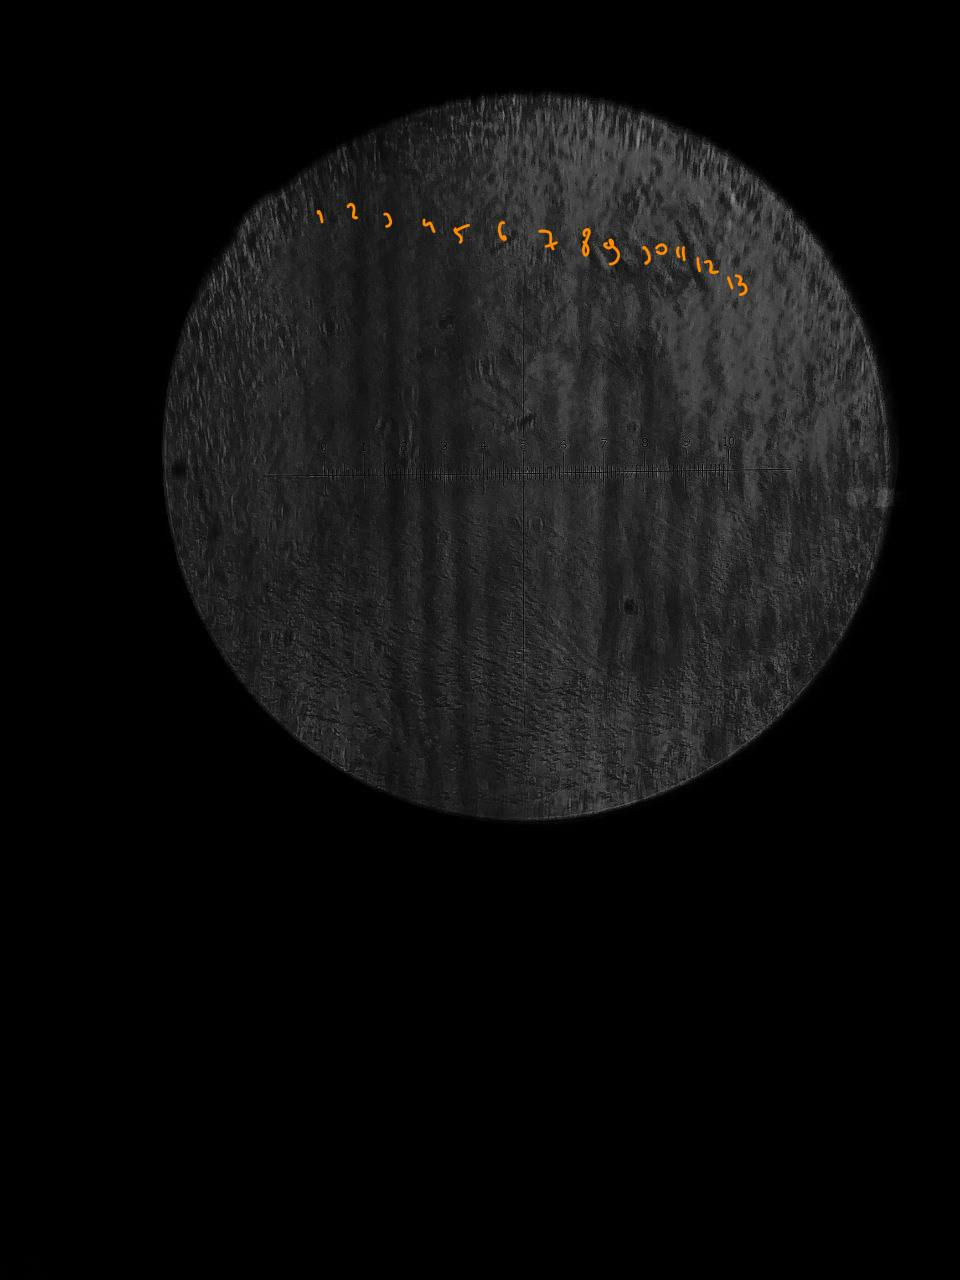
\includegraphics[width=0.7\textwidth]{grey 2.jpg}
	
	Наблюдаемая картина при частоте\\ 1.20 МГц в контрасте.
\end{center}
\end{minipage}


\end{enumerate}
\section{Обсуждение результатов ии вывод}
В работе была изучена дифракция света на акустической решетки, рассчитаны длина волны ультразвука и скорость его распространения в воде двумя способами: с помощью данных. полученных после измерения дифракционной картины и с помощью метода темного поля. Полученные результаты: $v=1591\pm52\text{ м/с}.$ (дифракция) и  $v = 1500 \pm 42 \text{ м/с} $ - темное поле, при табличном значении  $v=1490$ м/с.









\end{document}


